\documentclass{article}
\usepackage[margin=1in]{geometry}
\usepackage{url}
\usepackage{appendix}
\author{Ilkut Kutlar - u1621364}
\title{CS310 - Progress Report}
\usepackage{graphicx}
\begin{document}
	\maketitle
	\tableofcontents
	
	\newpage
	
	\section{Introduction}
	
	Synthetic Biology is a relatively new field concerned with creating new biological constructs not found in the nature with the aim of serving a useful purpose. The field involves an engineering process and therefore a researcher may need to go through a design stage before actually implementing the construct in a real organism. This project aims to make a CAD and simulation software for Gene Regulatory Networks (GRNs). The key and original ascpect of the software will be a reverse engineering feature which can change an existing circuit or create a new one to conform to a given list of constraints. This should be a useful feature for researchers and save time spent on manually designing a circuit with desired features.
	
		% Challenge?
	%- Quite a bit of research into Syn Bio -> Relatively new, so most resources are scientific papers.
	%- Syn Bio -> Simulation requires dealing with some maths, abstraction, algorithms.
	%- Rev. eng. requires quite a lot of maths
	%- Internal representation and program architecture: Need good design choices to make it maintainable.
	
	The challange with this project is both theoretical and practical. Given that synthetic biology is not a field I had encountered before, the theoretical challange is the significant research that goes into reading scientific papers to get an udnerstanding of the biology that lies behind the computer simulations, which is ultimately necessary to be able to interpret more complex scientific papers which assume a level of familiarity with biology, as well as papers describing various computational modelling and simulation methods necessary for the project. The practical challange is of implementing a complex system which aims to abstract and model a real life system. This requires good design choices to ensure a maintainable system is being developed. The final challange is of being able to implement the key feature of the system: reverse engineering of circuits. Implementing this feature will require mathematics and algorithmics skills.
	
	%TODO: Will require ... skills? Doesn't sound right...
	
	% TODO: Implementation part rather short? Could also include working with lbiraries and reading documentations, etc.
	
	\section{Background}
	

	
	The CAD of GRNs is useful for researchers, and thus this is a common problem. Some other similar tools include GenoCAD which allows design of GRNs
	
	...
	% TODO: Complete this
	
	
	% Background:
	% - It is a common problem, apparentlym so:
	% - There are similar toolds:
	%- GenoCAD for design & sim using COPASI
	%- TinkerCell
	%- COPASI
	
	\section{Progress}
	Out of all the objectives mentioned in the specification document and which should have been completed at this point, most have been completed while some components had to be changed and some parts of the timetable changed.
	
	% Improvements:
	
	%Work completed (eg: coding started; interviews set up; framework for
	%comparison of algorithms developed)
	%A list can be helpful - but do not just give a list
	%Again, do not just say you have done something. Evidence?
	%Check out the example project reports - how (well) do they
	%achieve this?
	
	\subsection{Final report} 
	The original timetable stated that starting from week 3, the final report would be updated continously as more features are added. This was eventually decided against as it is too early in the project and some details have not been clarified yet. Therefore, the writing of the final report will not start until term 2.
	
	\subsection{Testing} \label{progress-testing}
	The specification specified a unit test would be implemented for each objective. This could not be done because in their current states, the components making up the code are too large and thus not easily testable. In the next stage of the project, these components will be broken down into smaller subcomponents to allow easy testing.
	
	
	\subsection{Simulation model} 
	As mentioned in the specification, due to being ahead of schedule with the development progress, it was decided to switch to a more accurate and complex stochastic simulation model. 
	
	\subsection{Objective 1 (Models)}  
	The change in simulation model meant that the internal models used to represent a GRN had to be changed as well. Firstly, the stochastic simulation algorithm used works by randomly firing reactions. To account for this, a model for representing a reaction was added. Furthermore, the model for representing the whole system has been changed to a list of species which exist in the system and reactions which may occur at a given propensity and are in terms of the species of the system. Finally, the original plan modelled each genome as a collection of a promoter and coding regions. This would allow the user to create or import promoters and coding regions and build genomes modularly using the available parts. As the network is now a list of reactions and species, genomes are not modelled this way. In the new system, to build a genome obeying the properties of a given promoter and/or coding region, reaction rates can be changed.
	
	\subsection{Objective 2 (Simulation \& Visualisation)} 
	% TODO: Change this!
	
	This objective was changed slightly when the 
	After switching from an ODE to stochastic model, the original plan to do an ODE simulation was also updated to do a stochastic simulation. 
	
	The Gillespie algorithm used for stochastic simulation of the network have been implemented and can produce results. The visualisation of the produced results have also been implemented.
	
	\subsection{Objective 5a (User can add new parts)} 
	As explained before, as the system now is a list of species and reactions (and not genomes consisting a promoter and coding regions), the user now has to add reactions and supply reaction rates, rather than parts.
	% TODO: Maybe also add species?
	
	\subsection{Objective 6a (SBML parsing)} 
	This objective was originally planned for later on. However, it was decided to be implemented earlier, so that SBML models available online (for example on the Biomodels Database) could be easily imported into the software without having to manually enter values to allow convenient testing with other circuits. The SBML parsing was achieved using the \verb|libsbml| library. The parsed values are subsequently converted into the internal representation used by the program which can then be simulated. 
	% TODO: How do you prove correctness? Well, the manually entered values and the automaticly parsed one is more or less the same?
	
	
	\section{Design}		% Quality of design, does the system have a good design? This is the code stuff!
	
	
	\section{Choice of Methods and Tools}
	\begin{itemize}
		\item Python is used as the main development language. This was chosen as it is a very flexible language with an extensive range of mathematical and scientific libraries.
		\item The library \verb|matplotlib| \cite{matplotlib} was used for visualisation of simulation results. This is a popular library and thus has been thoroughly tested by many other users. The library is easy to use and offers many useful features out-of-the-box such as zooming into produced graphs, panning around, scaling, etc.
		\item For parsing SBML files, the \verb|libsbml| library was used. This library was developed by the original creators of the SBML standard and has excellent documentation, making it easy to work with.
		\item For designing the GUI, the \verb|GTK+ 3| library will be used. This was chosen over the more popular \verb|tkinter| library as \verb|GTK+ 3| has a more modern design and good documentation.
		\item For unit testing, the PyUnit library will be used.
		\item The current state of the software does not have a dependency on \verb|NumPy/SciPy| \cite{numpy, scipy} as was mentioned in the specification.
	\end{itemize}
	
	
	%Again, varies according to project type
	%- Development methods
	%- Technologies and languages
	%- Platforms, frameworks, datasets etc
	%- Project methodology (how you go about doing it)
	%- Data gathering methods
	%How are you doing things and what are you using to do these?
	
	%Progress:
	%- Models	-> Changed into reaction model
	%- Simulation & Visualisation	-> Changed to stochastic (as mentioned in spec)
	%- Half of SBML -> Why?
	%- How to prove they are done? Repressilator
	%- For each, say: Changes to original place, and current state.
	%- If not done, say why. With testing, not done because need to break it down further.
	
	\section{Project Management}
	\begin{itemize}
		\item Most of the important milestones mentioned in the original timetable have been achieved at this point. This success can mostly be attributed to the fact that the duration of all tasks were slightly overestimated.
		\item The experience gained during this first part of the project has lead to some changes having to be made to the original timetable:
		\begin{itemize}
			% TODO: Help with testing the system, good, but, elaborate?
			\item Tasks related to GUI have been decided to be of a greater importance than before due to its significance in determining usability. Starting the GUI earlier will allow more time to polish and improve it, as well as help with testing the system.
			\item The tasks related to the reverse engineering feature have been given more time. The extra time has been accounted for by parallelising the tasks with the GUI tasks. Doing so will be possible as this time period coincides with the Christmas holiday, during which some other commitments such as attending lectures, etc. will not continue, thus more time can be invested in the project.
			\item It has also been decided that a 10 day period will be allocated to researching and thinking about the type of approach to take for achieving reverse engineering and decide on the scope of the feature (i.e. which constraints will be offered).
			\item As mentioned in section \ref{progress-testing}, it was not possible to implement unit tests. To solve this problem, a 1 week period will be allocated to refactoring the current code to break it up into smaller, easily testable functions and write unit tests for each. The lessons learned from this experience will be used in the future to avoid the same problem with unit tests.
		\end{itemize}
		
	\end{itemize}
	
	\subsection{Updated Timetable}
	
	%% Updated timetable:
	%- Finally, the updated timetable: GUI and rev. eng. at the same time.
	%- Add a 1 week period for thinking about constraints.
	
	% Tech used:
	%- Python: Quick, elegant, and also very flexible. Proved very useful when passing around functions
	%- Matplotlib for visualisation -> Does everything out of the box, popular, stable
	%- Libsbml for parsing, but requires an adapter to convert into internal rep.
	%- GTK+ -> More modern than the de-facto standard of tkinter (Usability?)
	%- No more dependence on NumPy/SciPy for simulation/visualisation
	%- Needs some more refactoring to allow unit testing
	%- PyUnit for unit testing.
	
	% Project management:
	%- Scrum?
	%- Allowing more time than needed worked: I am now on track
	
	
	
	
	\newpage
	
	\appendix
	\appendixpage
	\addappheadtotoc
	
	% Include your specification here!

	\section{Problem Statement}
	
	\par Synthetic Biology is a relatively new and rapidly growing field focusing on biological constructs not found in nature. One specific area of focus is Genetic Regulatory Networks (GRNs), where the aim of researchers is to create useful genetic circuits capable of producing desired amounts of proteins, such as the Repressilator \cite{repressilator}, a novel circuit which produces three proteins at amounts which oscillate with time.
	% This has useful applications such as 
	\par Since Synthetic Biology deals with new circuits, there tends to be a design stage before the network is put together in a real organism. Computer Aided Design (CAD) can help accomplish this task.
	\par Some existing CAD and simulation software include COPASI\cite{copasi}, a tool for simulating biologcal reactions (not only related to GRNs). Another tool, GenoCAD\cite{genocad}, is a web-based software allowing design of genetic circuits from a database of parts, export it to some popular formats (such as SBML), and simulate the design using COPASI's API. TinkerCell\cite{tinkercell} is a similar desktop-based software, allowing drag-and-drop gene circuit design and simulation.
	\par This project will include features to design and simulate gene circuits, just as existing software do. One feature not offered by these software is reverse engineering of circuits, which this project will implement. This feature will allow the user to specify a set of constraints and properties (such as the required concentration of a certain product) and create a gene circuit having all the properties and obeying all the constraints. This has the potential of cutting down on the design time for a circuit and help researchers.
	%TODO: Why is this feature so useful? Elaborate more on this!
	
	% - (Some possible extensions:
	% - IDE functionality
	% - Calculation of values from sequences)
	
	
	% (Extra constraints could include: Do it in this organism, do it using only these parts, do it using so many parts, etc.)
	
	\section{Objectives}
	\par The software will let the user choose biological parts from a catalogue (which includes user generated parts as well as those fetched from a host of public databases), combine them (similar to building an electric circuit) and set the details of the relationship between them (such as the equations describing their regulatory relation). Software will then be able to simulate the circuit to allow observing the concentration of products over time. The key reverse engineering feature of the project will allow the user to state the desired amount of products and let the software reverse engineer a circuit capable of producing them. These objectives can be expressed more specifically as a list of main tasks, and a set of subtasks that needs to be completed for the main task to be complete:
	% TODO: I don't like the wording here
	
	\begin{enumerate}
		\item Should allow adding parts (as well as edit and delete them) to the network and specify their regulatory relations. Should allow the user to specify necessary network parameters.
		\begin{enumerate}
			\item Software should have a programmatic model of every supported part and its various parameters. This also includes non-trivial substances (which are not proteins or mRNA) which affect regulation, such lactose, as well as operons and other constructs which may be of importance to the process of regulation.
			\item Should keep track of the relations between each part (e.g. Which gene regulates a specific gene using which equation).
			\item Should store a programmatic model of the whole network, including parts, relations and global values. This subtask will build the foundation for the programmatic architecture of the project.
		\end{enumerate}
		
		\item Must be able to simulate the circuit.
		\begin{enumerate}
			\item Must be able to convert the programmatic model of the network into a series of mathematical equations which can be fed into an equation solver.
			\item Must solve the created equations and produce results (concentrations of products) at given intervals over a given period of time.
			\item Must be able to visualise the results of the simulation (e.g. using graphs).
		\end{enumerate}
		
		\item Must allow the user to specify a set of desired properties for the circuit to have (e.g. The amount produced of a certain protein should be above a certain number and the circuit should only use a given set of parts) and subsequently build a network which have these features.
		\begin{enumerate}
			\item Must convert the constraints given by the user into a set of mathematical constraints which the internal logic can work with.
			\item Needs to narrow down all possible circuit combinations to find the right one(s). 
		\end{enumerate}
		
		\item Must offer a user friendly UI.
		\begin{enumerate}
			\item Must visualise the circuit and its parts on the screen.
			\item Must allow drag-and-drop style interaction when adding and moving parts and defining relations between them.
			\item Must offer easy and intuitive access to parameters and values (such as clicking on a gene to access its associated parameters).
		\end{enumerate}
		
		\item It should be able to fetch biological parts (such as promoters, coding regions, etc.) and models (such as the Repressilator) from public databases (such as the BioModels\cite{biomodels} database, Registry of Standard Biological Parts \cite{rsbp}). Also needs to allow manuallly adding parts.
		\begin{enumerate}
			\item For some databases, needs to be able to scrape webpages.
			\item For some databases, needs to download machine-readable files and parse them.
			\item Needs to allow creation of parts from values entered by the user.
		\end{enumerate}
		
		\item Can import parts and models from a host of popular formats (such as SBML) and export to them.
		\begin{enumerate}
			\item Needs to be able to parse these formats.
			\item Needs to be able to convert the internal model used by this project to other popular formats.
		\end{enumerate}
		
	\end{enumerate}
	
	\subsection{Accuracy of the model}
	\par To be able to computationally represent a real Gene Regulatory Network (GRN), the software will have to adopt a mathematical model for GRNs. Researches have come up with various models of varying accuracy, ranging from boolean networks (which abstract some regulatory parameters) 
	% TODO: [CITE]
	to more accurate stochastic models (which aim to be accurate and take random noise into account as well).
	%TODO: [CITE]
	Furthermore, within each model, it is possible to abstract some factors which would have some effect on the process in real life. I am going to use Ordinary Differential Equations (ODEs) 
	%TODO: [CITE]
	to model the change in the concentration of mRNAs and proteins and model the gene regulation using Hill equation
	%TODO: [CITE]
	and take Hill coefficient to be 1. Finally, I will be considering the transcription rate, translation rate and mRNA and protein degradation rate for regulating transcription.
	
	\par However, it is possible that my chosen model may be too detailed and the time needed to implement it may cause me to miss some important milestones. On the contrary, it may be too abstract and not challenging enough. To avoid either problems, I have chosen a number of important dates (See the timetable section) on which I will consider my progress and decide whether I should revise my chosen model to make it more or less detailed.
	
	
	\section{Methods}
	
	\subsection{Software Methodology}
	%TODO This can be expanded
	\par I will be using a Scrum methodology, and in each sprint I will implement a new objective.
	
	
	\subsection{Version Management}
	\par For version management, I will be using Git, an open source software and will be pushing my changes to a remote private repository hosted at GitHub on my student account.
	
	\subsection{Evaluation \& Testing}
	\par I will be writing appropriate unit tests for each of the objectives apart from the ones related to a user friendly UI, as those cannot be tested with a unit test.
	\par To evaluate the circuit design and simulation features as a whole, I will build a network for which simulation results have been made available by other authors. The network will be using the same initial values, and the test will check whether my software produces the same results. 
	\par To evaluate the reverse engineering feature, I will input a set of constraints and let the software produce a circuit. Consequently, I will simulate the circuit in COPASI\cite{copasi}, an open source biological simulation software, and manually check whether the results obey the given constraints.
	
	\subsection{Timetable}
	
	\par I have prepared a Gantt chart to represent my plan for the project. I will be working on the final report all throughout the project, updating it as I add new features to the project. 
	
	\par During the "Biology Research" phase taking place at the beginning of the project, I will do some more reading on biology as I feel that improving my biology knowledge a little more will help with the project. The task names on the Gantt chart correspond to the ones listed in the Objectives section. 
	
	\par I planned for an "Extensions \& improvements" phase at the end. In the projects that I have done in the past, it usually was the case that after all the objectives were done, there were still some small bugs that needed fixing, as well as room for improvement and need for some polishing. Therefore, I wanted to leave some time at the end to make sure everything is working as expected. Furthermore, if things go as expected, I will also spend some time on implementing extensions which I didn't plan for due to time constraints.
	
	\par I purposefuly overestimated the time required for most tasks, as I know from my previous experiences that my estimates may sometimes be slightly inaccurate.
	
	\par Finally, as mentioned before, I plan to review my progress and revise the complexity of my biological model accordingly. I will do so on Week 9 of term 1, Week 3 of Term 2 and Week 8 of Term 2.
	
	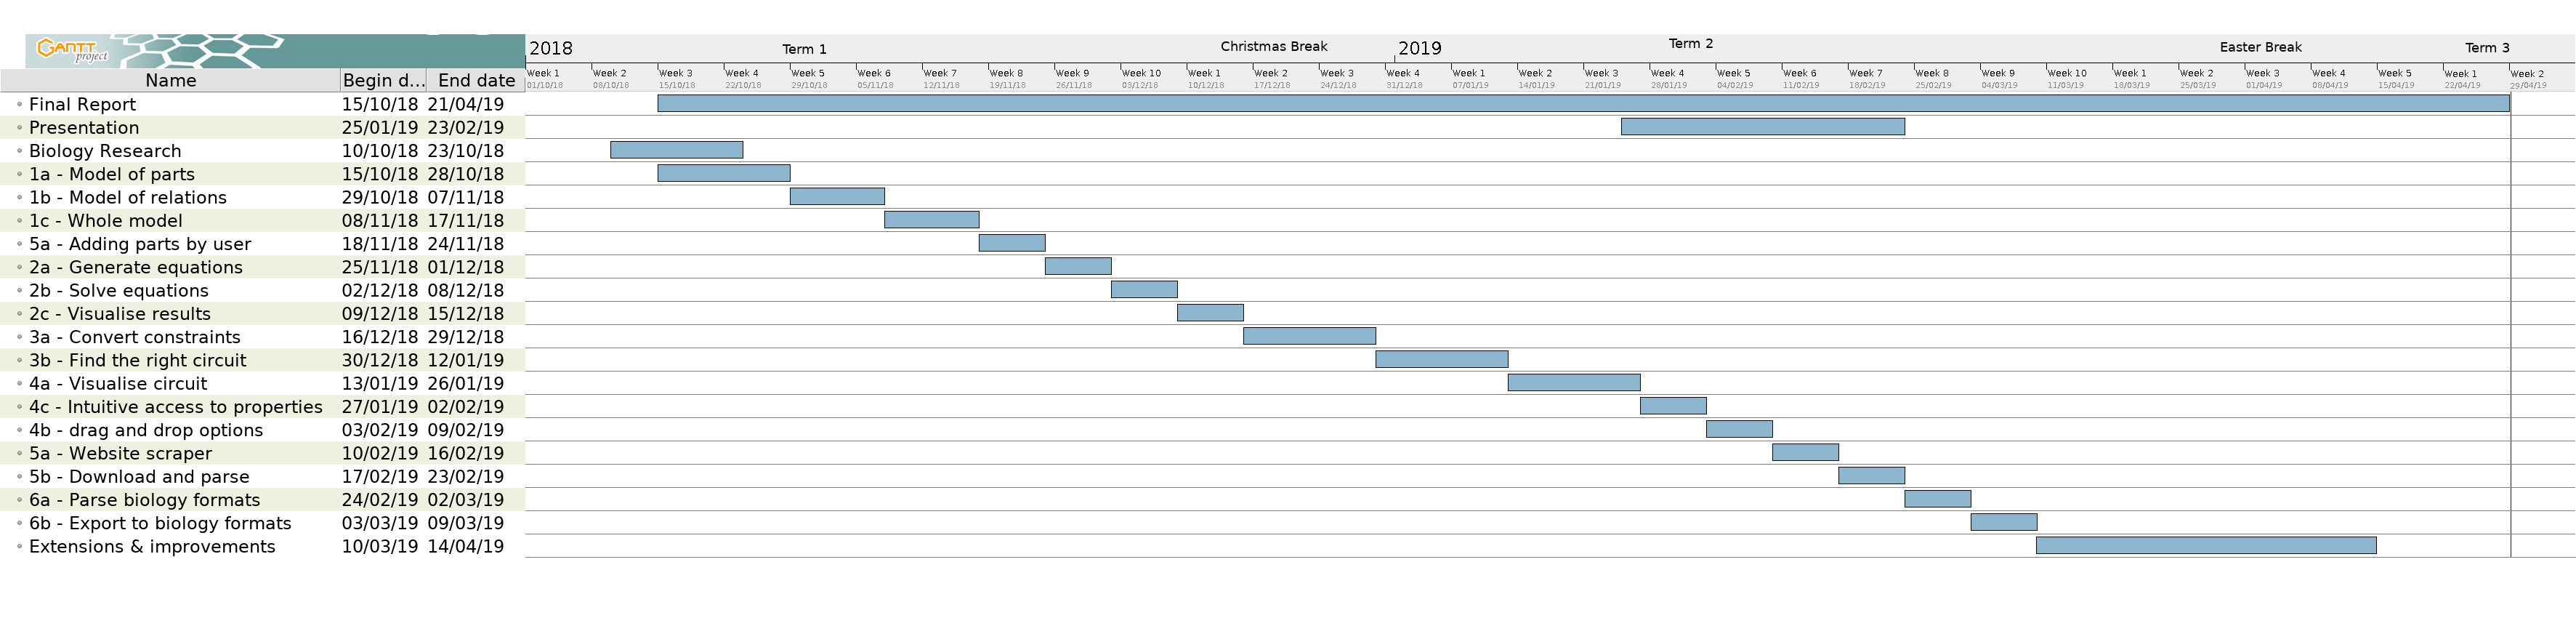
\includegraphics[height=120pt]{timetable}
	
	\section{Resources}
	\begin{enumerate}
		\item The software will be written in Python.
		\item The simulation feature will require libraries capable of handling mathematical operations. For this, I will be using NumPy \cite{numpy} and SciPy \cite{scipy}.
		\item For the visualisation of the simulation results, a graph plotting library will be required. For this, I will use matplotlib \cite{matplotlib}.
		\item Git \cite{git} and GitHub \cite{github} will be used for version control and backing up the software.
		\item The data required (for biological parts and models) will be fetched from public databases such as the BioModels \cite{biomodels} and the Registry of Standard Biological Parts. \cite{rsbp}
	\end{enumerate}
	
	\section{Risks}
	\paragraph{IT failure} I will be regularly pushing my local commits on Git to GitHub, a remote repository. Therefore, if my personal computer fails I can carry on working using departmental computers.
	\paragraph{Underestimation of the time required} In the case that I have not been able to complete some required tasks on time, leading to the project getting derailed, I will focus on the most essential features and not implement some non-essential features, such as having a user friendly UI.
	\paragraph{Unexpected problem preventing me from working for a period of time} To avoid such problems, I have overestimated the time required to complete tasks in my timetable.
	\paragraph{Working on assignments for other modules (especially when there will be many at the same time) may cause me to miss planned completion deadlines for this project's tasks} This may especially be a problem since the project will be running for a long time, which may cause me to lose focus and spend a disproportionate amount of time on other assignments. I have found that breaking down tasks into SMARTly defined subtasks help with keeping my focus, as I will know exactly what needs to be done.
	
	
	
	\section{Ethical Considerations}
	\begin{itemize}
		\item All software and services I plan to use (except GitHub) are free and open source and their licences do not restrict usages for a university dissertation project.
		\item GitHub normally charges a monthly fee for a private repository. However, as I have a student account, I am able to freely use a private repository.
		\item All data required for the software is publicly available.
	\end{itemize}
	
	\bibliographystyle{plain}
	\bibliography{progress}
\end{document}